\documentclass[
  aps,
  reprint,
  superscriptaddress,
  floatfix,
  nofootinbib,
  longbibliography
]{revtex4-2}

\usepackage{amsmath,amssymb}
\usepackage{graphicx}
\usepackage{xcolor}
\usepackage{tikz}
\usetikzlibrary{calc,positioning,arrows.meta}
\usepackage{hyperref}

\hypersetup{
  colorlinks=true,
  linkcolor=blue,
  citecolor=blue,
  urlcolor=blue
}

\newcommand{\R}{\mathbb{R}}
\newcommand{\E}{\mathbb{E}}
\newcommand{\Prob}{\mathbb{P}}
\newcommand{\T}{^{\mathsf T}}
\newcommand{\norm}[1]{\lVert #1\rVert}
\DeclareMathOperator{\Var}{Var}

\begin{document}

\title{Geometric Limits on Semantic Expressibility: Quantum-Inspired Contexts and Polysemy in Large Language Models}

\author{Karl Svozil}
\email{karl.svozil@tuwien.ac.at}
\affiliation{Institute for Theoretical Physics, TU Wien (Vienna University of Technology),
Wiedner Hauptstra\ss{}e 8--10/136, 1040 Vienna, Austria}

\date{\today}

\begin{abstract}
Why can next-token prediction produce language that appears meaningful?
Beginning with tokenization and vector encoding, we study two parts of this
question.  First, high-dimensional geometry permits exponentially many nearly
orthogonal feature directions at a fixed tolerance, although their residual
overlaps limit simultaneous readout.  Second, polysemy requires us to
distinguish static mixtures of word senses, context-dependent occurrence
vectors, neural feature superposition, quantum coherence, and one direction
shared by several orthonormal contexts.  The quantum comparisons are
structural and deliberately limited.  We end with an informal explanation of
self-attention, training, and autoregressive output; mathematical details are
relegated to undergraduate-level appendices.
\end{abstract}

\maketitle

% ======================================================================
\section{Why does a syntactic machine appear to understand?}
\label{sec:puzzle}
% ======================================================================

A large language model (LLM) receives strings and returns strings.  Yet it can
answer questions, continue an argument, translate a passage, and alter its
wording when the surrounding text changes.  In this behavioral sense it often
appears cognizant of what a text is about.  How can a machine trained to
predict linguistic form display abilities that we ordinarily describe in
terms of meaning?

The question recalls John Searle's Chinese Room thought experiment
\cite{searl-80a}.  A person who does not know Chinese follows formal rules for
transforming Chinese symbols and thereby produces answers that appear
intelligent to an outside reader.  Searle asks whether successful symbol
manipulation is sufficient for understanding.  We do not try to settle that
philosophical question, and fluent behavior will not be used as evidence of
consciousness.  Our question is narrower and operational: what internal
organization allows calculations on tokens to construct and exploit distinctions that
human readers recognize as semantic?

There is an important clue.  An LLM is not trained on arbitrary strings.
Its corpus was produced by people writing about objects, actions, intentions,
events, and one another.  Regularities of use therefore contain indirect
traces of regularities in human experience.  The model is never handed a
separate object called ``meaning.''  It is rewarded for predicting how
language is used.  Successful prediction can favor internal distinctions that
track the contexts in which words and constructions occur.  Whether this is
intrinsic understanding or a powerful simulation remains open; the present
chapter concerns the geometry of the representation.

Two issues provide a manageable route into that geometry.

First, a representation has a fixed number of independent coordinates, but it
may need to distinguish vastly more properties.  High-dimensional vector
spaces make this geometrically possible because they can contain very many directions that
are not exactly orthogonal but have small mutual overlaps.  We ask how this
\emph{quasi-orthogonality} enlarges expressive capacity and how accumulated
overlap---or interference---limits access to the stored distinctions.

Second, one word can have several meanings.  The word ``bank'' may refer to a
financial institution, the edge of a river, or a seat.  We ask how a single
token type and its many occurrences can represent such polysemy.  This leads
to comparisons with two different quantum ideas: coherent superposition and
one direction belonging to several orthonormal bases.

The order of exposition is intentional.  Section~\ref{sec:vectors} begins
with tokenization and explains why vector representations are useful.
Section~\ref{sec:quasi} develops the abundance--interference tradeoff in
informal terms.  Section~\ref{sec:polysemy} treats polysemy and the quantum
comparisons.  Only then does Sec.~\ref{sec:attention} open the Transformer and
explain attention, learning, and output generation.  Formal statements and
derivations appear in the appendices, where every symbol is defined as it is
introduced.

% ======================================================================
\section{From text to vectors}
\label{sec:vectors}
% ======================================================================

\subsection{Tokenization: symbols before geometry}

The first operation is \emph{tokenization}.  A tokenizer divides a character
string into units drawn from a finite vocabulary and replaces each unit by an
integer identifier.  A token may be a complete word, part of a word,
punctuation, a space-bearing fragment, or a byte-level unit.  Thus a token is
not automatically a word, still less a word's meaning.  Subword schemes
assemble rare and previously unseen words from reusable
fragments~\cite{sennrich2016subword}.

The assigned integer is merely an address.  Identifier 7193 is not
semantically closer to identifier 7194 than to identifier 20.  The identifiers
are therefore used as addresses in a table of vectors on which graded
comparison and learned transformation are possible.

\subsection{A token vector is a starting point, not a complete meaning}

A learned lookup table assigns a real vector to every token identifier.  Two
occurrences of the same identifier begin with the same table row.  The model
must also know order: ``the dog chased the cat'' is not equivalent to ``the
cat chased the dog.''  Position is therefore supplied in some form, either by
adding positional information or by altering comparisons inside attention.

The resulting initial vector is not a contextually complete meaning.  It has
been trained across many occurrences and can reflect what those occurrences
share, but later layers construct a new hidden vector for each particular
occurrence.  The occurrence of ``bank'' near ``loan'' can consequently acquire
a different hidden state from the same token near ``river,'' although both
began from the same lookup row.  This distinction between a token \emph{type}
and a contextual token \emph{occurrence} will be essential for polysemy.

\subsection{Why vectors?}

Vectors are useful for several reasons.  Their coordinates can be adjusted
continuously during learning.  Matrices can transform them and inner products
can compare them.  Vector addition permits several contributions to coexist
in one state.  Most importantly here, lengths, directions, projections, and
subspaces provide an economical language for graded features.

Suppose a unit vector $u$ has been fitted as a direction associated with some
property at a chosen layer.  The scalar $u\T h$ is then the signed coordinate
of a hidden state $h$ along that direction.  It is the coordinate, not the
axis itself, that says on which side of the contrast the state lies and how
strongly.  In a simplified gender example, [[let one orientation or subspace spanned by a vector, encode gender. O]]ne may orient a fitted axis from
a feminine-marked sample mean toward a masculine-marked sample mean.  Positive
and negative projections then describe opposite sides of the same fitted
contrast; they are not two orthogonal directions.  A midpoint or probe
intercept must define the zero.  Modern contextual representations may use
several related directions rather than one universal axis, and the score can
change from sentence to sentence
\cite{bolukbasi2016gender,zhao2019contextualgender}.  The superscript
$\mathsf T$ means transpose, so $u\T h$ is the ordinary Euclidean inner
product.

This directional interpretation is operational, not metaphysical.  It depends
on the layer, data, centering, inner product, and extraction method. [[ A probe
that reads a property does not by itself prove that the model uses the same
direction causally.  Nor does perpendicularity prove that two concepts are
unrelated---??? contradictory to independence?]].  Orthogonality has one precise consequence for a linear readout:
[[\textit{semantic independence} of the respective concepts, as
a component along one direction [[representing one concept]] contributes no cross-talk when the other [[concept orr feature]] is
read by an inner product.

The reason to emphasize vectors is therefore not that meanings are known in
advance to be points in a Euclidean space.  It is that a trained vector system
can discover useful graded distinctions, combine them, and compare them by
simple operations.  High dimension adds a striking opportunity: far more
approximately separated directions can coexist than there are exactly
independent coordinates.  That opportunity motivates our first central
issue.

% ======================================================================
\section{Many directions in a fixed-width space}
\label{sec:quasi}
% ======================================================================

\subsection{Exact independence and approximate separation}

In a $d$-dimensional space, no more than $d$ nonzero vectors can be mutually
orthogonal.  This is elementary linear algebra: mutually orthogonal nonzero
vectors are linearly independent, and a linearly independent family cannot
contain more vectors than the dimension.  If semantic distinctions required
exactly perpendicular axes, fixed width would impose a severe limit.

Exact orthogonality is stronger than most readouts require.  Let $u$ and $v$
be unit vectors.  Their inner product is the cosine of the angle between them.
We call them quasi-orthogonal at tolerance $\varepsilon$ when
$|u\T v|\leq\varepsilon$, where the tolerance is chosen before the comparison.
They are not independent coordinates; they are approximately separated
directions.

High-dimensional geometry makes such directions surprisingly abundant.
For a uniformly random unit vector in $d$ real dimensions, the overlap with a
fixed unit direction is typically of size $1/\sqrt d$.  Most of the sphere is
therefore concentrated near the equator perpendicular to any chosen
direction.  L\'evy's concentration principle expresses this typicality.
The Johnson--Lindenstrauss lemma approaches the same phenomenon from another
side: a finite collection of points can be placed in a dimension proportional
to the logarithm of the number of points while approximately preserving all
pairwise distances.  Read in the constructive direction, these results show
that at any fixed nonzero angular tolerance a $d$-dimensional representation
space admits
at least exponentially many quasi-orthogonal directions
\cite{ledoux2001concentration,johnson-1984,Dasgupta-2003}.

The word \emph{exponential} is important, but so are its qualifications.  It
counts directions available at the chosen tolerance, not a second
vector-space dimension.  It is a geometric possibility, not proof that a
trained model uses all those directions.  The allowed overlap must be stated,
and an exponentially large dictionary is not automatically readable when
many of its elements are active at once.  Appendix~\ref{app:geometry} gives
the concentration, union-bound, and Johnson--Lindenstrauss calculations. [[please refer to Appendix \label-for-A earlier]]

\subsection{The price of abundance: interference}

The simplest calculation already shows the access problem.  Suppose a hidden
state contains two unit feature directions,
\begin{equation}
 h=a u+b v.
 \label{eq:two-feature-main}
\end{equation}
Reading the first feature by an inner product gives
$u\T h=a+b(u\T v)$.  The desired coefficient is $a$; the second term is
cross-talk from the other feature.  Exact orthogonality removes it, while
quasi-orthogonality bounds its size by $\varepsilon|b|$.

Many small unwanted terms can nevertheless accumulate.  If $k$ comparably
sized, random-like features are active and their signs do not align
systematically, their mean squared errors add as in the Pythagorean theorem.
The resulting root-mean-square (RMS) interference is of order
$\sqrt{k/d}$ relative to one unit-scale target.  This is an average random-code
benchmark, not a guarantee for every learned dictionary.  In the worst case,
aligned cross-terms can add rather than cancel.

The useful operating region is consequently task dependent.  There should be
enough distinguishable directions for the features a task needs, but not so
many simultaneously active, strongly overlapping directions that the chosen
readout fails.  There is no universal numerical boundary determined by $d$
alone.  It also depends on which features coactivate, their strengths, the
decoder, and the tolerated error.  A learned model may use its angular budget
selectively, placing greater separation between features that frequently need
to be read together.

\subsection{A limited analogy with geometric decoherence}

Small overlaps also occur in quantum theory.  When alternatives of a quantum
system become correlated with nearly orthogonal environmental states, the
off-diagonal terms of the reduced state are multiplied by the corresponding
environmental overlaps.  High dimension can make those factors very small
when the conditional states or their relative dynamics satisfy an explicit
typicality assumption; dimension alone is not enough, since the conditional
states could remain identical.  The author's companion analysis studies this
purely geometric contribution to decoherence
\cite{svozil2026geometricdecoherence}. [[---please quote as https://doi.org/10.48550/arXiv.2605.03807 ]]

The LLM analogy is narrow.  Quasi-orthogonal semantic directions suppress
linear cross-talk in much the way that nearly orthogonal environmental branch
states suppress observable coherence terms.  We call this \emph{geometric
decoherence}: unwanted contributions become small because the relevant inner
products are small.  It is not physical quantum decoherence.  An LLM has no
required system--environment split, unitary branch dynamics, partial trace,
or local loss of access to phase relations after environmental degrees of
freedom are traced out.  High dimension supplies shared geometry, not a
shared physical mechanism
\cite{RevModPhys.75.715}.

The word \emph{orthogonal} also has different operational meanings here.  For
the LLM readout it means [[semantic independence and ]]absence of linear cross-talk in the chosen inner
product.  Within one quantum measurement context, orthogonal rays represent
mutually exclusive outcomes.  The common inner-product geometry does not make
these interpretations identical.

This qualified comparison is still useful.  In both settings, exact
orthogonality is an ideal limit; approximate orthogonality can already make
alternatives operationally difficult to confuse; and the number of pairwise
small overlaps is not the same as the number of alternatives that can be
reliably recovered together.

% ======================================================================
\section{Polysemy: one form, several meanings}
\label{sec:polysemy}
% ======================================================================

\subsection{A sense is not a single feature}

[[Present encoding of semantic polysemy is in terms of a classical real-valued convex summation---not a quantum complex superposition---of vectors contributing.
]]

A \emph{sense} is a contextually appropriate meaning of a lexical item.  The
financial, river-edge, and seat meanings of ``bank'' are different senses.
The banking or tilting of an aircraft supplies another.  A semantic feature is
narrower: it may mark animacy, tense, number, sentiment, or one fitted gender
contrast.  Several features can contribute to one sense, and one feature can
recur in many words and senses.  Polysemy is therefore not solved merely by
finding one direction for every dictionary definition.

It is also important to say which representation is being discussed.  A
static embedding assigns one stored vector to a word type.  A transformer has
one initial lookup row for a token type but constructs different hidden
vectors for its occurrences.  These are related but not identical problems.

\subsection{A static vector as a corpus-level mixture}

In a static system such as word2vec, the same stored type vector is used in
every occurrence.  [[In contradistinction, ]]under a particular generative model, Arora and
collaborators establish an approximate relation between that vector
and hypothetical sense vectors \cite{arora-etal-2018-linear}.  The following
three-sense equation illustrates the corresponding finite-mixture idea:
\begin{equation}
\begin{aligned}
 &v_{\rm bank}\approx
 p_{\rm fin}v_{\rm fin}
 +p_{\rm river}v_{\rm river}
 +p_{\rm seat}v_{\rm seat},\\
 &p_{\rm fin},p_{\rm river},p_{\rm seat}\ge� 0,\\
 &p_{\rm fin}+p_{\rm river}+p_{\rm seat}=1 .
\end{aligned}
 \label{eq:static-mixture-main}
\end{equation}
The nonnegative coefficients  summarize how frequently the senses occur in the
corpus.  The equation is an approximate classical convex combination and a
population-level summary.  It does not decide what one occurrence means, nor
does one observed sum uniquely determine its hidden summands.

Arora et al. also expressed each word vector using only a few reusable,
topic-like directions, which they called discourse atoms.  This sparse
description can help recover recurring components across many words.  It does
not show that all sense vectors or atoms are mutually quasi-orthogonal, and
the atoms need not correspond
one-to-one with dictionary senses.  The geometric results of
Sec.~\ref{sec:quasi} establish what is possible at a chosen tolerance; they do
not establish what a learned lexical dictionary actually contains.

[[ please delete entirely if not essential. Oterewise tell me, and completely rewrite without technical blurbs

\subsection{Contextual occurrences}

Modern transformers begin each occurrence of a token type from the same
lookup row, apart from positional treatment, but the available sequence
changes the subsequent calculation.  The financial and river occurrences of
``bank'' can therefore acquire different hidden vectors.  In a causal
decoder, the state at a position uses only the prefix available there.  If a
disambiguating word follows ``bank,'' the earlier state for ``bank'' cannot
see it, although later positions can combine both words.  The phrase
``surrounding context'' must be understood with that causal qualification.

A simple interpretable model would let the available text reweight several
sense vectors.  A real transformer is not required to implement that literal
mixture.  Its layers apply learned linear maps, nonlinear transformations,
residual additions, and attention.  Ambiguous sentences and puns may also
preserve information relevant to more than one sense.  It is therefore safer
to say that contextualization \emph{transforms} an occurrence representation
than that it selects or collapses one pre-existing branch.

The phrase \emph{neural feature superposition} denotes yet another classical
idea.  A hidden state may contain a sum of many feature directions, with a
sparse subset appreciably active on a particular input
\cite{elhage2022superposition,bricken2023monosemanticity}.  The coefficients
may be signed and need not add to one; the features need not be word senses.
Thus a static lexical mixture, a contextual occurrence state, and neural
feature superposition are three different objects.

]]

\subsection{Why this is not automatically quantum coherence}

Quantum theory uses the word \emph{superposition} in a stronger operational
sense.  A pure state combines alternatives with [[complex and thus not necessarily convex]] probability amplitudes.
Relative phase can affect later measurement probabilities when alternatives
are recombined in another basis, and the Born rule turns amplitudes into
probabilities.  A classical frequency average such as
Eq.~\eqref{eq:static-mixture-main} provides none of this.  Its coefficients are
frequencies, not amplitudes; no phase-sensitive transformation or interference
experiment is specified; and its sense vectors are not declared orthonormal
measurement outcomes.

Why not impose a full quantum-style superposition?  One may certainly propose
a new mathematical model that does so.  But the proposal would have to state
the sense basis, amplitudes, relative phases, allowed transformations,
measurement rule, and an experiment in which phase changes alter observable
predictions.  Without those ingredients, replacing the classical weights by
symbols resembling quantum amplitudes merely renames a vector sum.  Existing
Transformer attention supplies no Born rule and no physical collapse.  The
explicit pure-state and density-matrix comparison is given in
Appendix~\ref{app:polysemy}.

\subsection{A different quantum analogy: shared contexts}

Quantum logic suggests a comparison that does not rely on vector addition.
An orthonormal measurement context can be represented by mutually orthogonal
rays, or equivalently by rank-one projectors that sum to the identity.  In
dimension at least three, distinct contexts may contain the same projector
while differing in their other members.  This is an incidence relation: one
element belongs to several contexts.

The diagram below borrows that pattern for a speculative representation of
``bank.''  Its center is a fixed lexical projector.  Each colored arm belongs
to a different larger context, whose remaining directions carry
context-specific information.  The same lexical element is retained, while
the financial, river-edge, and seat contexts differ around it.

\begin{figure}[t]
\centering
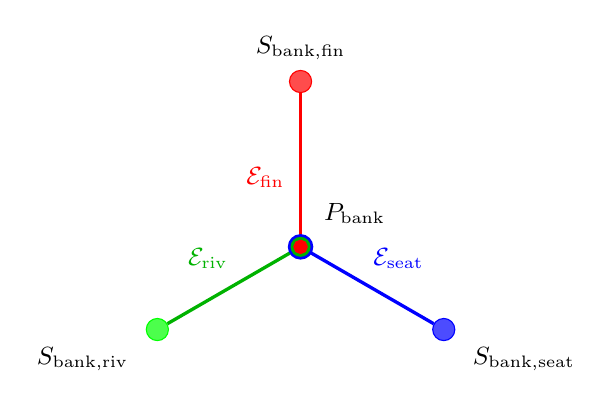
\begin{tikzpicture}[scale=0.5,
    outer/.style={circle, draw, minimum size=8pt,
                  inner sep=0pt, font=\footnotesize},
    lab/.style={font=\small}]
% central shared reference-subspace vertex
\coordinate (c) at (0,0);

\node[lab, above right=7pt] at (c)
{$P_{\rm bank}$};

% outer sense-subspace vertices
\node[outer, red, fill=red!70,
      label={[lab]above:
      $S_{{\rm bank},{\rm fin}}$}]
      (fin) at (90:4.2cm) {};

\node[outer, green, fill=green!70,
      label={[lab, xshift=-4pt]below left:
      $S_{{\rm bank},{\rm riv}}$}]
      (riv) at (210:4.2cm) {};

\node[outer, blue, fill=blue!70,
      label={[lab, xshift=4pt]below right:
      $S_{{\rm bank},{\rm seat}}$}]
      (seat) at (330:4.2cm) {};

% hyperedges labelled by context
\draw[very thick, red] (c) --
      node[lab, left=2pt, pos=0.45]
      {$\mathcal E_{\rm fin}$} (fin);

\draw[very thick, green!70!black] (c) --
      node[lab, above left=1pt, pos=0.45]
      {$\mathcal E_{\rm riv}$} (riv);

\draw[very thick, blue] (c) --
      node[lab, above right=1pt, pos=0.45]
      {$\mathcal E_{\rm seat}$} (seat);

% central concentric disks
\filldraw[blue, very thick] (c) circle (8pt);
\filldraw[green!70!black, very thick] (c) circle (6pt);
\filldraw[red, very thick] (c) circle (4pt);
\end{tikzpicture}
\caption{Structural incidence schematic for ``bank.''  The central projector
$P_{\rm bank}$ is shared.  Each colored arm shows only a fragment of one
context hyperedge; unshown orthogonal projectors complete the corresponding
basis.  An outer node $S_{{\rm bank},s}$ summarizes a residual semantic sector,
not necessarily one rank-one outcome.  The drawing depicts shared incidence,
not the vector sum in Eq.~\eqref{eq:static-mixture-main}.}
\label{fig:contexts}
\end{figure}

This analogy has a sharp limit.  The shared projector alone cannot say which
sense is intended.  If a quantum system were prepared exactly in that shared
ray, a measurement in any basis containing it would return the shared outcome
with certainty.  More generally, for a fixed quantum state the Born
probability of the same projector does not depend on which compatible
projectors complete the basis.  Linguistic interpretation is different in the
relevant respect: it is supposed to depend on the available text.

The diagram can therefore motivate only an optional classical hypothesis: a
contextual occurrence vector might retain a stable nonzero lexical component
while placing sense-dependent information in accompanying directions.  Such a
decomposition is mathematically easy to construct; its scientific content
would lie in stability, predictive usefulness, and improvement over simpler
untied contextual models.  The analogy is structural, not a claim that
polysemy is a quantum measurement.  Appendix~\ref{app:polysemy} gives the
shared-projector construction and explains why quantum probability rules do
not transfer to linguistic context.


[[ I would completely eliminate these entire sectiosn ...

% ======================================================================
\section{What is established, what is proposed, and how it could fail}
\label{sec:tests}
% ======================================================================

This chapter reports no new experiment.  It combines established mathematics
with empirical hypotheses, and that distinction should remain visible.

The geometric statements are established.  At a fixed nonzero tolerance,
high-dimensional spheres admit exponentially large families of directions
with bounded pairwise overlap.  Uniformly random pairs have RMS overlap
$1/\sqrt d$.  For a specified linear correlation readout, overlap produces the
cross-term displayed in Eq.~\eqref{eq:two-feature-main}.  These facts say
nothing by themselves about which semantic features an LLM has learned.

The first empirical question is therefore whether feature directions
extracted by a declared method show useful geometry on held-out data.  Their
overlaps should be compared with isotropic random controls and with
activity-matched controls.  The most relevant overlaps are those between
features that coactivate and need to be read together.  Failure to beat these
baselines would weaken the claim that learning has allocated angular
separation strategically.

The second question concerns polysemy.  An Arora-style static mixture should be
tested in one declared lexical space with sense frequencies estimated from
training data.  A contextual representation should then predict held-out
senses or same-sense judgments better than that static prior.  Otherwise the
contextual account has added complexity without demonstrated benefit.

The third question concerns the optional shared anchor in
Fig.~\ref{fig:contexts}.  It must be learned on training data, remain
non-negligible and stable on held-out occurrences, and improve prediction,
compression, or sample efficiency relative to equally flexible models without
the shared-anchor constraint.  Since any chosen vector can be completed to an
orthonormal basis, merely drawing several contexts around one ray is no
evidence.  If the anchor becomes negligible, varies strongly with context, or
fails against simpler controls, this optional proposal should be rejected
while the ordinary contextual account remains intact.

No such test establishes consciousness, intrinsic intentionality, or a
physical quantum process.  The measurable claims concern representation,
overlap, readout, and predictive behavior.

% ======================================================================
\section{How attention uses context and produces text}
\label{sec:attention}
% ======================================================================

We have so far treated the transformer---a layered neural-network architecture
centered on attention---as a device that changes an initial token vector into
a context-dependent occurrence vector.  We now return to that missing
mechanism.  The informal account needs only vectors, matrices, inner products,
weighted averages, and smooth nonlinear transformations.

\subsection{Two meanings of ``weight''}

The word \emph{weight} is used for two different things.  The embedding table
and the matrices inside attention, feed-forward, and output blocks are
\emph{persistent model parameters}.  Training changes them, and the resulting
numbers survive from one prompt to the next.  Self-attention also computes
temporary, input-dependent numbers commonly called attention weights.  To
avoid confusion, we call the latter \emph{attention coefficients}.  They are
recomputed for every sequence, layer, head, and permitted target--source pair
of positions.  Attention does not itself create the persistent model
parameters.

\subsection{Self-attention as context-dependent routing}

At a given layer, every token position carries a current hidden vector.  One
attention head applies three learned linear maps to these vectors.  Their
outputs are conventionally called queries, keys, and values.  The query and
key are two transformed views used to calculate a match score; the value is
the transformed content routed according to that score.  The names are
mnemonics rather than literal mental operations.

For one target position, the head compares its query with the keys at the
positions it is allowed to inspect.  Inner products supply the comparison
scores.  A text-generating, decoder-only model uses a causal mask, so it cannot
inspect future tokens.  Softmax normalization turns the permitted scores into
nonnegative
attention coefficients whose sum is one.  The head then forms a weighted
average of the corresponding value vectors
\cite{Vaswani-2017-Attention}.

This weighted average is only the immediate output of one head.  A practical
layer combines several heads.  An output map combines their results; a
residual connection adds the layer's input back; and a feed-forward block is
a small nonlinear network applied at each position.  The complete layer is
therefore neither a mere average nor an orthogonal projection.
Repeated layers allow the representation at one position to gather and
transform information from many permitted positions.

For ``bank,'' evidence such as ``deposit,'' ``loan,'' and ``interest'' can
create different query--key matches and value contributions than ``river,''
``water,'' and ``shore.''  At the position of ``bank,'' a causal model can use
only evidence already in the prefix; evidence appearing later can be combined
with ``bank'' only at later positions.  Attention thereby participates in
contextualization and may retain, combine, or later discard several kinds of
evidence.

\subsection{How training learns the persistent parameters}

During language-model training, the network sees a token sequence and is
asked at each permitted position to predict the following token.  One sequence
therefore supplies many prediction examples: the state at position $i$
predicts the token at position $i+1$.  Because the causal mask prevents access
to later tokens, the eligible distributions can be computed in parallel
during one forward pass.  A loss is large when the continuation that actually
occurred received little probability and small when it received much
probability.

Backpropagation applies the multivariable chain rule to determine how the loss
changes when each persistent parameter changes.  An optimizer then adjusts
the parameters slightly to lower the current minibatch loss.  Repeating the
forward--loss--backward--update cycle over many varied text segments aims to
improve prediction on unseen continuations and produces the trained model
\cite{Goodfellow-et-al-2016-Book}.

Self-attention matters during this process because the error is differentiated
through its query, key, value, and softmax calculations.  Nevertheless, in
each individual forward pass the persistent matrices are fixed.  Attention
produces contextual activations and temporary coefficients; gradient-based
optimization produces the trained parameter values.

\subsection{Autoregressive output}

When a trained model answers a prompt, its persistent parameters normally
remain fixed.  The prompt is tokenized, mapped to initial vectors, and passed
through the transformer.  An output map converts the final-layer hidden state
at the last position of the current prefix into one score for every token in
the vocabulary.  Softmax turns those scores into a distribution over possible
next tokens; it is not a probability that the completed statement is true.
A decoding rule either chooses a
high-scoring token or samples from a selected portion of that distribution
\cite{Brown2020May}.

The chosen identifier is appended to the prefix.  The enlarged prefix becomes
the input for the following prediction, so one generated token can change all
later hidden states and attention coefficients.  The model ordinarily does
not compose a complete answer in a hidden store and then reveal it.  It
constructs the response one token at a time.  Finally, detokenization joins
the generated pieces into readable text.

This loop is recursive in its state but not usually in its persistent
parameters: output becomes new input, while the deployed weights remain
unchanged.  External memory or retrieval can also change later inputs without
changing the model.  Genuine online learning would be a separate
parameter-update procedure, not ordinary autoregression.

The calculation now closes the conceptual loop.  The model never receives a
dictionary entry called ``meaning.''  It receives token occurrences in human
text, turns them into vectors, and learns transformations that improve
prediction.  Some of the resulting geometry supports distinctions and
contextual responses that readers interpret semantically.  This explains a
plausible, testable route to meaning-sensitive behavior without deciding whether the machine
understands in Searle's philosophical sense.

... until here!]]

% ======================================================================
\section{Conclusion}
\label{sec:conclusion}
% ======================================================================

Searle's Chinese Room asks whether correct manipulation of symbols amounts to
understanding.  We have not answered that philosophical question.  We have
instead followed one operational path from tokens to meaning-sensitive
behavior.

Token identifiers first become vectors because vectors support graded
coordinates, learned transformations, comparison, and combination.  Their
high-dimensional geometry addresses the first problem considered here.  A
fixed-width representation space can accommodate exponentially many quasi-orthogonal
directions at a chosen tolerance, even though it has only $d$ exactly
independent coordinates.  This is expressive room, not cost-free access.
Residual overlaps create interference, especially when many relevant features
are active together.

The resulting overlap suppression has a limited quantum counterpart.  Small
inner products suppress cross-terms both in linear semantic readout and in
the environmental overlaps that enter quantum decoherence.  The shared
geometry justifies the phrase geometric decoherence, while the absence of
quantum dynamics, relative phases, and environmental tracing prevents a physical
identification.

Polysemy exposes different limits of the quantum comparison.  A static word
vector may approximate a frequency-weighted convex mixture of sense vectors,
and a transformer constructs context-dependent occurrence vectors.  Neither
is thereby a coherent quantum superposition, and attention is not collapse.
The star diagram retains only a quantum-logical incidence idea: one lexical
projector may be shared by several orthonormal contexts.  That optional
constraint must earn its place empirically; the common ray alone does not
select a meaning.

Attention finally explains how available tokens affect one another's
representations, training explains how prediction errors change persistent
parameters, and autoregression explains how vectors are converted back into a
sequence of tokens.  Together these mechanisms outline a plausible route by
which syntactic prediction can acquire a geometry useful for semantic
discrimination.
[[ At the moment quantum mechanics appears to bear only superficial resemblence with LLMs: they
both share Hilbert space; but  different ones n terms of scalars and encoding structures such as contexts,
or coherence and interference.
Some aspects pertain in both formalisms; in particular, when it comes to quasi-orthogonality wich in
LLM is the basis of semantic richness, and in quantum mechanics mayimpress quasi-classicality of macro-events.]]

\appendix

% ======================================================================
\section{Formal companion to \emph{From text to vectors}}
\label{app:vectors}
% ======================================================================

This appendix gives a minimal mathematical version of
Sec.~\ref{sec:vectors}.  It distinguishes strings, token identifiers, and
vectors before discussing semantic directions.

\subsection{Tokenization and lookup}

Let $\mathcal S$ be the set of finite character strings.  Let
$\mathcal V=\{1,\ldots,V\}$ be a vocabulary containing $V$ token identifiers.
Each identifier is an integer label.  A tokenizer is a fixed map
\begin{equation}
 \mathsf{Tok}:\mathcal S\longrightarrow
 \bigcup_{T\geq0}\mathcal V^T.
 \label{eq:tokenizer-app}
\end{equation}
If $\mathsf{Tok}(\sigma)=(t_1,\ldots,t_T)$, then the input string $\sigma$
has become a sequence of $T$ identifiers.  The union in
Eq.~\eqref{eq:tokenizer-app} allows strings to produce sequences of different
lengths.  A detokenizer reverses the assembly, subject to the system's stated
normalization rules.

Let $d_{\rm model}$ be the architectural width of the model's hidden stream.
The notation $\R^m$ means the set of real column vectors with $m$ coordinates.
An embedding table is a real matrix
$E\in\R^{V\times d_{\rm model}}$.  Its row $E[t_i]$ is the initial lookup
vector for identifier $t_i$.  In a simple additive positional scheme,
\begin{equation}
 h_i^{(0)}=E[t_i]+p_i,
 \qquad h_i^{(0)},p_i\in\R^{d_{\rm model}}.
 \label{eq:lookup-app}
\end{equation}
Here $p_i$ supplies the position and the superscript $(0)$ means the stage
before the first transformer layer.  Some architectures encode position by
rotating queries and keys rather than literally adding $p_i$; the conceptual
role is the same.  The identifier $t_i$, the table row $E[t_i]$, and the
contextual state produced at a later layer are three different objects.

The geometric analysis need not use all $d_{\rm model}$ architectural
coordinates.  A declared preprocessing map may center the observed states and
remove nearly unused directions.  It may also rescale the retained principal
directions to a declared common variance, a step called whitening.  We use
$d\leq d_{\rm model}$ for the rank of the resulting representation space.
Any numerical claim involving $d$ must therefore report the model,
layer, sample, centering, rank threshold, and inner product used to obtain it.

\subsection{Projection onto a fitted feature direction}

Let $u\in\R^d$ be a unit vector, so $u\T u=1$.  The orthogonal projection of a
state $h$ onto the line through $u$ is
\begin{equation}
 P_u h=(u\T h)u,
 \qquad P_u=uu\T .
 \label{eq:projection-app}
\end{equation}
The scalar $u\T h$ is its signed coordinate.  The matrix $P_u$ is called a
projector because direct multiplication gives $P_u^2=P_u$.  The remainder
$h-P_u h$ is perpendicular to $u$, since
$u\T(h-P_u h)=0$.  This is the elementary orthogonal projection theorem in
finite-dimensional form.

An oriented contrast needs a baseline.  Suppose two training samples have
means $\mu_A$ and $\mu_B$ in the same representation space and
$\mu_A\ne\mu_B$.  Define
\begin{equation}
\begin{aligned}
 g&=\frac{\mu_A-\mu_B}{\norm{\mu_A-\mu_B}},
 &h_0&=\frac{\mu_A+\mu_B}{2},\\
 \alpha_g(h)&=g\T(h-h_0).
\end{aligned}
 \label{eq:signed-axis-app}
\end{equation}
The unit vector $g$ orients the contrast, $h_0$ declares its midpoint, and
$\alpha_g(h)$ is the signed coordinate.  Substitution shows
\begin{equation}
 \alpha_g(\mu_A)=\frac{\norm{\mu_A-\mu_B}}{2},
 \qquad
 \alpha_g(\mu_B)=-\frac{\norm{\mu_A-\mu_B}}{2}.
 \label{eq:mean-scores-app}
\end{equation}
Swapping the two groups reverses $g$ and every sign but does not change the
unoriented line.  A score near zero means that the coordinate along $g$ is near
the midpoint; it does not imply that the full vector is near $h_0$, because a
large perpendicular component may remain.

The same construction can illustrate a fitted gender-associated contrast,
but it does not define gender and need not capture all gender-related
information.  A linear classifier provides a related alternative: if its
decision boundary is $w\T h+\beta_0=0$ with $w\ne0$, then
$(w\T h+\beta_0)/\norm w$ is signed Euclidean distance from that hyperplane.
Either construction must be fitted on training examples and evaluated on
held-out examples.

% ======================================================================
\section{Formal companion to the geometric argument}
\label{app:geometry}
% ======================================================================

The main text used three counts.  The integer $d$ is the exact dimension of
the selected vector space.  The integer $M$ is the number of feature or code
directions in a declared dictionary.  The integer $k$ is the number of those
directions appreciably active in one state.  Only $d$ is a vector-space
dimension.

\subsection{Exact orthogonality and quasi-orthogonality}

Let $w_1,\ldots,w_M\in\R^d$ be unit vectors.  The family is
$\varepsilon$-quasi-orthogonal when
\begin{equation}
 |w_i\T w_j|\leq\varepsilon
 \quad\hbox{whenever }i\ne j,
 \qquad 0<\varepsilon<1.
 \label{eq:quasi-app}
\end{equation}
The absolute value treats a direction and its negative as the same
unoriented axis for purposes of overlap.

When $\varepsilon=0$, the vectors are mutually orthogonal.  To see why there
can then be at most $d$, suppose
$a_1w_1+\cdots+a_Mw_M=0$.  Taking the inner product with $w_j$ leaves
$a_j=0$, because every cross-term vanishes and $w_j\T w_j=1$.  All
coefficients are zero, so the vectors are linearly independent.  The
definition of dimension now gives $M\leq d$.

For $\varepsilon>0$, the vectors need not be linearly independent.  The
largest possible $M$ becomes a finite spherical-code problem at the chosen
tolerance.  Its cardinality is sometimes informally called
quasi-dimensionality, but no additional linear dimensions have appeared.

\subsection{Why typical overlaps shrink with dimension}

For a random quantity $Y$, $\E[Y]$ denotes its average.  For an event $A$,
$\Prob(A)$ denotes its probability.  A unit vector chosen uniformly from the
sphere has no preferred direction: rotating the whole experiment does not
change its probability law.

Fix a unit vector $u$ and choose $X$ uniformly from the unit sphere in
$\R^d$.  Rotational symmetry lets us take $u$ to be the first coordinate
direction.  The overlap $u\T X$ is then $X_1$.  Symmetry makes all coordinate
squares have the same expectation.  Since
$X_1^2+\cdots+X_d^2=1$, taking expectations gives
\begin{equation}
 1=d\,\E[X_1^2],
 \qquad
 \E[(u\T X)^2]=\frac1d.
 \label{eq:rms-overlap-app}
\end{equation}
The RMS overlap is the square root of the mean squared overlap, hence
$1/\sqrt d$.  This elementary calculation gives a scale, not a tail
probability and not a guarantee for learned vectors.

L\'evy's concentration lemma supplies the tail.  One convenient consequence
is that universal positive constants $c$ and $C$ exist such that
\begin{equation}
 \Prob\{|u\T X|>\varepsilon\}
 \leq C\exp(-c d\varepsilon^2)
 \label{eq:levy-overlap-app}
\end{equation}
for a fixed unit $u$ and a relevant fixed tolerance.  The function
$x\mapsto u\T x$ is 1-Lipschitz because the Cauchy--Schwarz inequality gives
$|u\T(x-y)|\leq\norm{x-y}$.  L\'evy's lemma says that a Lipschitz function on
a high-dimensional sphere is unlikely to deviate far from its typical value.
Here 1-Lipschitz means that changing the input by a distance $r$ changes the
function value by at most $r$
\cite{ledoux2001concentration,milman1986asymptotic}.

\subsection{From one pair to an exponential family}

Choose $M$ directions independently and uniformly.  There are
$M(M-1)/2$ unordered pairs.  The union bound states that the probability of at
least one bad pair is no larger than the sum of the bad-pair probabilities.
Combining it with Eq.~\eqref{eq:levy-overlap-app} gives
\begin{equation}
 \Prob\!\left\{
 \max_{i\ne j}|w_i\T w_j|>\varepsilon
 \right\}
 \leq \frac{C M(M-1)}{2}
 \exp(-c d\varepsilon^2).
 \label{eq:union-app}
\end{equation}
Choose the greatest integer $M$ not exceeding
$\exp(c'\varepsilon^2d)$, where $c'$ is sufficiently small and $d$ is
sufficiently large.  Then the right side is below one.  Therefore at least one
family of that exponential size has every overlap within tolerance.  This is
an existence lower bound and a random-code benchmark, not a universal maximum
and not proof that an LLM learns such a code.

Solving the exponent in Eq.~\eqref{eq:union-app} for the overlap tolerance
shows that the union-bound crossover is a constant multiple of
$\sqrt{\log M/d}$ when $\log M$ is small compared with $d$.  The union bound
supplies a high-probability upper scale, not by itself a matching lower law.
This remains a null-model estimate rather than a hard capacity wall.

\subsection{The Johnson--Lindenstrauss route}

The Johnson--Lindenstrauss lemma states that a set of $M+1$ points can be mapped
into $\R^d$ while preserving all squared distances within relative error
$\delta$ when
\begin{equation}
 d\geq C_{\rm JL}\delta^{-2}\log(M+1),
 \qquad 0<\delta<1,
 \label{eq:jl-app}
\end{equation}
where $C_{\rm JL}$ is a numerical constant and $\log$ is the natural logarithm
\cite{johnson-1984,Dasgupta-2003}.  This is a theorem about a prescribed finite
set, not random semantic features.

To obtain a quasi-orthogonal code, take the origin and $M$ mutually orthogonal
standard coordinate vectors $e_i$ in a sufficiently large starting space.
Let $\Phi$ be a linear Johnson--Lindenstrauss map and define
$y_i=\Phi e_i$.  Including the origin controls the image lengths.  The
polarization identity
\begin{equation}
 2y_i\T y_j=\norm{y_i}^2+\norm{y_j}^2-\norm{y_i-y_j}^2
 \label{eq:polarization-app}
\end{equation}
turns preservation of lengths and distances into preservation of inner
products.  Before normalization their pairwise absolute inner products are at
most $2\delta$; because every squared length is at least $1-\delta$, the
normalized overlaps are at most $2\delta/(1-\delta)$.  For a fixed target
dimension $d$, choose an integer $M$ satisfying
$M+1\leq\exp(c\delta^2d)$, with $c$ small enough that
Eq.~\eqref{eq:jl-app} holds.  This constructs an exponential-size family.

L\'evy concentration, random spherical coding, and the
Johnson--Lindenstrauss lemma are thus related views of one high-dimensional
phenomenon.  Their exponential factors must not be multiplied as though they
were independent mechanisms.

\subsection{A deterministic overlap floor}

Random coding gives a typical construction.  The Welch bound gives a
deterministic limitation.  Put the vectors into the columns of a matrix
$W\in\R^{d\times M}$ and form the Gram matrix $G=W\T W$.  Its entry
$G_{ij}=w_i\T w_j$ records every pairwise overlap.  The diagonal entries are
one, so the trace of $G$ is $M$.  The matrix has rank at most $d$ and
nonnegative eigenvalues.

Let $\lambda_1,\ldots,\lambda_r$ be its nonzero eigenvalues, where $r\leq d$.
Cauchy--Schwarz gives
\begin{equation}
 M^2=\left(\sum_{\ell=1}^r\lambda_\ell\right)^2
 \leq r\sum_{\ell=1}^r\lambda_\ell^2
 \leq d\sum_{\ell=1}^r\lambda_\ell^2.
 \label{eq:eigen-cs-app}
\end{equation}
The sum of squared matrix entries equals the sum of squared eigenvalues for a
real symmetric matrix.  Removing the $M$ diagonal ones and averaging the
remaining entries yields
\begin{equation}
 \max_{i\ne j}|w_i\T w_j|^2
 \geq \frac{M-d}{d(M-1)}
 \qquad (M>d).
 \label{eq:welch-app}
\end{equation}
This is the Welch bound \cite{welch1974coherence}.  It says that once the
dictionary is overcomplete, some nonzero overlap is unavoidable.  It does not
say which pair overlaps or how damaging that pair is for a particular task.

\subsection{Two-feature and many-feature readout}

Let a hidden state be represented by
\begin{equation}
 h=\sum_{i\in A}a_iw_i+e.
 \label{eq:feature-code-app}
\end{equation}
Here $A$ is the active set, $a_i$ are scalar feature coefficients, and $e$ contains
components omitted by this chosen dictionary.  Reading feature $j\in A$ by
correlation gives
\begin{equation}
 w_j\T h
 =a_j+\sum_{\substack{i\in A\\i\ne j}}
 a_i(w_j\T w_i)+w_j\T e.
 \label{eq:readout-app}
\end{equation}
The first term is desired; the sum contains geometric cross-talk.
Equation~\eqref{eq:two-feature-main} is the case $A=\{1,2\}$ and $e=0$.

If the directions are $\varepsilon$-quasi-orthogonal, the triangle inequality
gives the worst-case bound
\begin{equation}
 \left|
 \sum_{\substack{i\in A\\i\ne j}}a_i(w_j\T w_i)
 \right|
 \leq\varepsilon\sum_{\substack{i\in A\\i\ne j}}|a_i|.
 \label{eq:worst-readout-app}
\end{equation}
This bound allows every unwanted term to have the same sign.  Under a
different, explicitly random-like model, assume instead that the cross-terms
are centered, have zero cross-moments, and satisfy
$\E[(w_j\T w_i)^2\mid w_j]=1/d$.  Treat the active set and coefficients as fixed
and condition on $w_j$.  Variances then add:
\begin{equation}
 \E\!\left[
 \left.
 \left(\sum_{\substack{i\in A\\i\ne j}}a_iw_j\T w_i\right)^2
 \right|A,(a_i),w_j
 \right]
 =\frac1d\sum_{\substack{i\in A\\i\ne j}}a_i^2.
 \label{eq:variance-readout-app}
\end{equation}
For $k-1$ interfering features of comparable unit coefficient, the square root
is $\sqrt{(k-1)/d}$.  This is the RMS law quoted in the main text.  Centering
or zero cross-moments is essential; an informal claim of uncorrelated
contributions would be insufficient without their means being defined.

The contrast between Eqs.~\eqref{eq:worst-readout-app} and
\eqref{eq:variance-readout-app} explains why no universal Goldilocks boundary
follows from $d$ and $M$ alone.  A task must also specify active coefficients,
coactivation frequencies, a decoder, and an accepted error.  Overlap between
two features that never need to be recovered together may have little cost.

\subsection{The common algebra behind geometric decoherence}
\label{app:dirac}

We first introduce the notation used in this comparison.  A quantum state is
a complex column vector.  Dirac notation writes such a vector as a
\emph{ket} $|v\rangle$ and its conjugate transpose as the \emph{bra}
$\langle v|$.  Thus $\langle v|w\rangle$ is an inner product, whereas
$|v\rangle\langle w|$ is a matrix called an outer product.  A density matrix
is a positive semidefinite matrix of trace one; the trace is the sum of its
diagonal entries.  The partial trace over an environment is the linear
operation that discards the environmental coordinates while preserving all
expectation values of measurements made only on the system.

For comparison with physical decoherence, let
$\{|s_i\rangle\}$ be orthonormal alternatives of a quantum system.  Suppose a
system--environment interaction produces the pure joint state
\begin{equation}
 |\Psi\rangle=\sum_i c_i\,|s_i\rangle|E_i\rangle,
 \qquad \sum_i|c_i|^2=1.
 \label{eq:branch-state-app}
\end{equation}
The normalized $|E_i\rangle$ are conditional environmental states.  Observing
only the system means taking a partial trace over the environment.  The
reduced system state is
\begin{equation}
 \rho_S
 =\sum_{i,j}c_i c_j^*
 \langle E_j|E_i\rangle\,|s_i\rangle\langle s_j|.
 \label{eq:reduced-state-app}
\end{equation}
Thus every off-diagonal term with $i\ne j$ is multiplied by an environmental
overlap.  When the relevant $|E_i\rangle$ become nearly orthogonal, those
coherence terms become small for system-only observations.  This is the
standard algebraic core of environmental decoherence
\cite{RevModPhys.75.715}.

Near-orthogonality of the $|E_i\rangle$ requires a stated assumption about the
interaction or branch-state ensemble; high dimension alone does not produce
it.  Moreover, many small off-diagonal terms can accumulate.  Therefore,
bounding each pair separately does not by itself show that the whole reduced
matrix is close to the matrix obtained by deleting all off-diagonal terms.

Compare Eq.~\eqref{eq:reduced-state-app} with
Eq.~\eqref{eq:readout-app}.  The quantum coherence term is suppressed by
$\langle E_j|E_i\rangle$; the classical readout error is suppressed by
$w_j\T w_i$.  Both are small-overlap effects.  Only the former follows from a
joint quantum state and a partial trace.  The latter is ordinary cross-talk in
a real linear readout.  This is why geometric decoherence is an analogy in the
LLM setting rather than a claim of physical decoherence.

\subsection{Conditional tensor-product amplification}

One further scaling is mathematically correct but not implied for an ordinary
transformer.  If a separate model genuinely has $n$ tensor factors, each of
fixed local dimension $q\geq2$, then its exact Hilbert-space dimension is
\begin{equation}
 d=q^n.
 \label{eq:tensor-dimension-app}
\end{equation}
Substitution into the exponential code bound gives
\begin{equation}
 M\geq\exp(c\varepsilon^2q^n)-1,
 \label{eq:double-exponential-app}
\end{equation}
which is doubly exponential in the number of factors $n$ at fixed $q$ and
$\varepsilon$, for sufficiently large $n$.  This is a code cardinality, not
an additional Hilbert-space dimension.  A real code is also a valid subset of
the corresponding complex representation space.  Standard LLM residual width
is not known to equal an accessible $q^n$ tensor-product representation space, so
Eq.~\eqref{eq:double-exponential-app} is not an ordinary LLM capacity claim.

% ======================================================================
\section{Formal companion to the polysemy comparison}
\label{app:polysemy}
% ======================================================================

\subsection{Static mixture, contextual reweighting, and feature code}

Let $t$ denote a word type, or a token that corresponds to a complete lexical
item, and let $s\in\{1,\ldots,S_t\}$ index its candidate senses.  Let
$v_{t,n}^{\rm type}$ be the static embedding estimated from an amount of corpus
data indexed by $n$.  Under the generative assumptions used by Arora et al.,
this estimate converges in the corpus limit to a population vector $\bar v_t$.
That limit is approximately related to sense-specific embeddings
$q_{t,s}$ by
\begin{equation}
\begin{aligned}
 v_{t,n}^{\rm type}&\longrightarrow\bar v_t &&(n\to\infty),\\
 \bar v_t&\approx\sum_{s=1}^{S_t}\pi_t(s)q_{t,s},
 &\qquad \sum_s\pi_t(s)&=1.
\end{aligned}
 \label{eq:arora-app}
\end{equation}
If $f_{t,s}$ is the corpus count of sense $s$ among occurrences of type $t$,
then $\pi_t(s)=f_{t,s}/\sum_r f_{t,r}$ is its relative frequency.  The first
relation is the asymptotic convergence statement; the second is the
model-dependent approximation to a frequency-weighted sense sum.  Arora et
al.\ prove the displayed relation explicitly for two senses; the finite
multisense expression is their general linearity assertion and follows from
the same conditioning argument \cite{arora-etal-2018-linear}.  Keeping the two
relations separate avoids attributing every modeling residual to finite-sample
error.

An interpretable contextual extension replaces the fixed frequency prior by
weights inferred from the available text $x$:
\begin{equation}
\begin{aligned}
 q_t^{\rm mix}(x)
 &=\sum_{s=1}^{S_t}p_\theta(s\mid x,t)q_{t,s},\\
 p_\theta(s\mid x,t)&\geq0,
 &\sum_s p_\theta(s\mid x,t)&=1.
\end{aligned}
 \label{eq:context-mixture-app}
\end{equation}
The subscript $\theta$ denotes fitted parameters of the contextual weighting
rule.  Equation~\eqref{eq:context-mixture-app} is a useful classical baseline.
An actual transformer guarantees only that some learned map $F_\ell$ produces
an occurrence state
\begin{equation}
 h_\ell(t\mid x)=F_\ell(E[t],x)
 \label{eq:context-state-app}
\end{equation}
at layer $\ell$.  It need not implement the explicit convex mixture in
Eq.~\eqref{eq:context-mixture-app}.

A general neural feature code has still another form:
\begin{equation}
 h_\ell(t\mid x)
 =b_\ell+\sum_{i=1}^{M}a_i(t,x)w_i+e_\ell(t,x).
 \label{eq:neural-superposition-app}
\end{equation}
Here $b_\ell$ is a baseline, $w_i$ are learned or extracted feature
directions, $a_i$ are input-dependent activations, and $e_\ell$ is the
unmodeled residual.  The $a_i$ may be signed and need not sum to one.  Only a
subset may be appreciably active.  Thus Eq.~\eqref{eq:neural-superposition-app}
is a linear decomposition of an activation, not a probability mixture of word
senses.

\subsection{Quantum pure superposition and incoherent mixture}

Using the Dirac notation introduced in Appendix~\ref{app:dirac}, let
$\{|s\rangle\}$ now denote orthonormal quantum alternatives.  A normalized
pure state is
\begin{equation}
 |\psi\rangle=\sum_s c_s|s\rangle,
 \qquad
 \sum_s|c_s|^2=1.
 \label{eq:pure-superposition-app}
\end{equation}
The coefficients $c_s$ are amplitudes.  They may be real or complex; quantum
coherence does not require every amplitude to be non-real.  What matters is
that relative signs or phases can affect probabilities after a change of
measurement basis.

The density matrix of the pure state is
\begin{equation}
 |\psi\rangle\langle\psi|
 =\sum_{s,r}c_s c_r^*|s\rangle\langle r|.
 \label{eq:pure-density-app}
\end{equation}
The star denotes complex conjugation.  Terms with $s\ne r$ are off-diagonal
coherences in this basis.  By contrast, an incoherent quantum state formed by
classical probabilistic mixing of the same orthogonal alternatives is
represented by
\begin{equation}
 \rho_{\rm mix}=\sum_s p_s|s\rangle\langle s|,
 \qquad p_s\geq0,\quad\sum_s p_s=1.
 \label{eq:density-mixture-app}
\end{equation}
This positive semidefinite, trace-one matrix has no off-diagonal terms in the
displayed basis.  Under its intended lexical interpretation, the Arora sum in
Eq.~\eqref{eq:arora-app} is neither
Eq.~\eqref{eq:pure-superposition-app} nor
Eq.~\eqref{eq:density-mixture-app}: it is a real vector average in a lexical
embedding space.  Ordinary Euclidean cross-terms do not establish quantum
interference.

\subsection{The optional shared-projector construction}

Let $r_t\in\R^d$ be a unit lexical anchor and let
\begin{equation}
 P_t=r_t r_t\T
 \label{eq:lexical-projector-app}
\end{equation}
be its rank-one projector.  For linguistic context class $s$, choose
$m_s$ orthonormal residual directions perpendicular to $r_t$ and place them
in the columns of
\begin{equation}
\begin{aligned}
 B_{t,s}&=
 [u_{t,s,1}\ \cdots\ u_{t,s,m_s}],\\
 B_{t,s}\T B_{t,s}&=I_{m_s},
 &B_{t,s}\T r_t&=0.
\end{aligned}
 \label{eq:residual-basis-app}
\end{equation}
The identity matrix $I_{m_s}$ has $m_s$ rows and columns.  The columns of
$B_{t,s}$ form an orthonormal partial frame.  The Gram--Schmidt or
orthonormal-extension theorem permits it to be completed to a full basis of
$\R^d$.  Put $P_{t,s,j+1}=u_{t,s,j}u_{t,s,j}\T$ for the displayed residual
directions and use the additional basis directions for the remaining
projectors.  In projector language, a completed context has the form
\begin{equation}
 \mathcal E_{t,s}
 =\{P_t,P_{t,s,2},\ldots,P_{t,s,d}\},
 \qquad
 P_t+\sum_{j=2}^{d}P_{t,s,j}=I_d.
 \label{eq:context-hyperedge-app}
\end{equation}
The $P_{t,s,j}$ are mutually orthogonal rank-one projectors.  Different
hyperedges $\mathcal E_{t,s}$ may share $P_t$ and differ in their other
projectors.  The orthonormal completion is nonunique, so its mere existence is
automatic mathematics rather than an empirical discovery.

A strict shared-anchor hypothesis for contextual states could be written
\begin{equation}
\begin{aligned}
 h_\ell(t\mid x)
 &=a_t r_t+B_{t,s(x)}z_{t,s(x)}(x)\\
 &\quad+e_t(x),\\
 P_t e_t(x)&=0,\\
 B_{t,s(x)}\T e_t(x)&=0.
\end{aligned}
 \label{eq:shared-anchor-app}
\end{equation}
Here $s(x)$ is a context class inferred from text, $z_{t,s(x)}(x)$ contains
context-dependent residual coordinates, and $a_t\ne0$ is required to be the
same across contexts.  The two displayed orthogonality conditions put
$e_t(x)$ outside both the anchor and the selected residual sector, so
components cannot be shifted arbitrarily between $B_{t,s(x)}z_{t,s(x)}(x)$
and $e_t(x)$.  Only the component $a_t r_t$ is fixed; the complete
occurrence vector generally changes.  If the entire vector were fixed, the
context would have to be stored elsewhere and that vector alone would not
encode polysemy.

For a fixed quantum state $\rho$, the Born probability assigned to the shared
projector is
\begin{equation}
 p(P_t\mid\rho)=\operatorname{tr}(\rho P_t).
 \label{eq:born-shared-app}
\end{equation}
No term in this expression names the other projectors that complete the
measurement context.  Gleason's theorem, under its additivity hypotheses in
real or complex dimension at least three, derives this density-operator form
for projector probabilities \cite{Gleason}.  This limited probability
consistency does not say that quantum mechanics admits a global
noncontextual assignment of sharp values.  The Kochen--Specker theorem rules
out such assignments under its own assumptions \cite{specker-60,kochen1}.
Neither theorem implies that linguistic context should obey a Born rule.

% ======================================================================
\section{Formal companion to attention, training, and output}
\label{app:attention}
% ======================================================================

Let $\Theta$ denote all persistent model parameters: the embedding table,
attention and feed-forward matrices, normalization parameters, and vocabulary
readout.  During one forward pass $\Theta$ is fixed.  Hidden states, queries,
keys, values, and attention coefficients are transient quantities computed
from the current sequence.

\subsection{One causal attention head}

Let $h_i\in\R^{d_{\rm model}}$ be the current hidden vector at target position
$i$.  Let $d_h$ be the width of one attention head.  Three learned matrices
$W_Q,W_K,W_V\in\R^{d_h\times d_{\rm model}}$ produce
\begin{equation}
 q_i=W_Qh_i,\qquad
 k_j=W_Kh_j,\qquad
 v_j=W_Vh_j.
 \label{eq:qkv-app}
\end{equation}
The vectors $q_i$, $k_j$, and $v_j$ are the query at target position $i$ and
the key and value at source position $j$.

In a decoder-only causal model, position $i$ may use positions $j\leq i$.  The
scaled score, attention coefficient, and one-head aggregate are
\begin{align}
 s_{ij}&=\frac{q_i\T k_j}{\sqrt{d_h}},\nonumber\\
 \alpha_{ij}
 &=\frac{\exp(s_{ij})}
 {\sum_{r=1}^{i}\exp(s_{ir})},\nonumber\\
 a_i^{\rm att}&=\sum_{j=1}^{i}\alpha_{ij}v_j.
 \label{eq:attention-app}
\end{align}
The factor $1/\sqrt{d_h}$ keeps the scale of the scores roughly stable.  If
coordinate products have comparable variance, adding $d_h$ of them makes an
unscaled dot product's typical size grow like $\sqrt{d_h}$.
The exponential is positive, so every $\alpha_{ij}\geq0$, and direct
summation shows $\sum_{j=1}^i\alpha_{ij}=1$.  Thus the immediate aggregate of
one head is a convex combination of its permitted value vectors.  The complete
multi-head block subsequently applies output maps and a residual connection,
so the whole transformer layer need not be a convex combination or a
projector.

The Cauchy--Schwarz inequality gives
$|q_i\T k_j|\leq\norm{q_i}\norm{k_j}$.  A large score therefore requires
appropriate alignment and scale.  The learned matrices decide which aspects
of the incoming states become relevant to the comparison.

\subsection{Next-token probabilities and training}

After the final layer $L$, let $h_i^{(L)}$ be the contextual state at position
$i$.  Let $W_{\rm out}\in\R^{V\times d_{\rm model}}$ and $b\in\R^V$ be the
vocabulary readout matrix and bias.  The score vector $g_i\in\R^V$ and the
probability of candidate token $a\in\mathcal V$ are
\begin{align}
 g_i&=W_{\rm out}h_i^{(L)}+b,\nonumber\\
 p_\Theta(a\mid t_1,\ldots,t_i)
 &=\frac{\exp(g_{i,a})}
 {\sum_{c\in\mathcal V}\exp(g_{i,c})}.
 \label{eq:output-softmax-app}
\end{align}
The entries of $g_i$ are scores, often called logits.  The softmax denominator
makes the probabilities nonnegative and makes them sum to one over the
vocabulary.

For a training sequence $(t_1,\ldots,t_T)$ with $T\geq2$, the standard
next-token negative log-likelihood is
\begin{equation}
 \mathcal L(\Theta)
 =-\sum_{i=1}^{T-1}
 \log p_\Theta(t_{i+1}\mid t_1,\ldots,t_i).
 \label{eq:loss-app}
\end{equation}
Each term is small when the observed next token received high probability.
Backpropagation applies the multivariable chain rule to compute the gradient
$\nabla_\Theta\mathcal L$.  The elementary gradient step
\begin{equation}
 \Theta_{\rm new}
 =\Theta-\eta\nabla_\Theta\mathcal L,
 \qquad \eta>0,
 \label{eq:gradient-app}
\end{equation}
changes the persistent parameters.  At a point where the loss is
differentiable, the first-order Taylor formula explains the minus sign:
\begin{equation}
 \mathcal L(\Theta-\eta\nabla\mathcal L)
 \approx\mathcal L(\Theta)
 -\eta\norm{\nabla\mathcal L}^2.
 \label{eq:taylor-app}
\end{equation}
For a nonzero gradient and a sufficiently small step, the linear term lowers
the same loss locally.  Practical optimizers add batching, adaptive scaling,
momentum, regularization, and other refinements; the separation remains:
attention computes transient coefficients, while optimization updates
persistent parameters.

\subsection{Autoregressive generation}

Let $(u_1,\ldots,u_m)$ be the tokenized prompt, where $m$ is its length, and
let $\Theta^\star$ be the deployed parameters.  Here the star labels the
chosen deployment checkpoint; it is not complex conjugation.  After
processing a current
prefix $(u_1,\ldots,u_j)$, the model produces scores $g_{j,a}$ for the next
token.  With a positive decoding temperature $\tau_{\rm dec}$, define
\begin{equation}
 \pi_j(a)=
 \frac{\exp(g_{j,a}/\tau_{\rm dec})}
 {\sum_{c\in\mathcal V}\exp(g_{j,c}/\tau_{\rm dec})},
 \qquad \tau_{\rm dec}>0.
 \label{eq:generation-softmax-app}
\end{equation}
Lower temperature magnifies score differences and concentrates the
distribution; higher temperature makes it flatter.  Temperature changes the
sampling distribution, not the learned scores themselves.
The next identifier $u_{j+1}$ is selected from $\pi_j$ by the declared
decoding rule and appended to the prefix:
\begin{equation}
 (u_1,\ldots,u_j)
 \longmapsto
 (u_1,\ldots,u_j,u_{j+1}).
 \label{eq:autoregressive-app}
\end{equation}
The enlarged prefix is processed again for the following token.  During
ordinary inference $\Theta^\star$ stays fixed; the prefix, hidden states, and
attention coefficients change.  Detokenization assembles the generated
identifiers into the final character string.

Online adaptation would be a separate learning procedure and lies outside the
present scope.

\begin{acknowledgments}
OpenAI Codex using GPT-5 (generative pre-trained transformer, version 5) was
used to assist with literature organization, \LaTeX{}
editing, and checks of derivations.  The author specified the scientific
direction and prompts; model output retained in the manuscript was checked
against the cited sources and explicit calculations.  The author accepts full
responsibility for the final text.

This research was funded in part by the Austrian Science Fund (FWF), grant
digital object identifier (DOI)
\href{https://doi.org/10.55776/PIN5424624}{10.55776/PIN5424624}.
The author also acknowledges support from the TU Wien Bibliothek Open Access
Funding Programme.

The author declares no conflict of interest.
\end{acknowledgments}

\bibliography{svozil}

\end{document}
